\documentclass[12pt]{report}
\usepackage[a4paper,left=25.4mm, right=25.4mm, top=25.4mm, bottom=25.4mm]{geometry}
\usepackage[utf8]{inputenc}
\usepackage{graphicx}

%list/enum
\usepackage{outlines}

%code
\usepackage{listings}
\usepackage{color}
\usepackage{inconsolata}
 
\definecolor{codegreen}{rgb}{0,0.6,0}
\definecolor{codegray}{rgb}{0.5,0.5,0.5}
\definecolor{codepurple}{rgb}{0.58,0,0.82}
\definecolor{backcolour}{rgb}{0.95,0.95,0.92}
\definecolor{comments}{rgb}{0,0.3,0}
 
\lstset{language=Go,
    backgroundcolor=\color{backcolour},  
    basicstyle=\ttfamily\footnotesize,
    keywordstyle=\color{blue}\ttfamily,
    stringstyle=\color{red}\ttfamily,
    commentstyle=\color{comments}\ttfamily,
    breakatwhitespace=false,         
    breaklines=true,                 
    captionpos=b,                    
    keepspaces=true,                 
    numbers=left,                    
    numbersep=5pt,                  
    showspaces=false,                
    showstringspaces=false,
    showtabs=false,                  
    tabsize=2
}
 

%titlesec and titleformat for chapters without 'chapter 1' tags
\usepackage{titlesec} 
\titleformat{\chapter}[display]
  {\normalfont\bfseries}{}{0pt}{\Huge}

%for clickable table of contents
\usepackage{hyperref}
\hypersetup{
    colorlinks,
    citecolor=black,
    filecolor=black,
    linkcolor=black,
    urlcolor=black
}

%for glossary of terms
\usepackage[acronym]{glossaries}
\makeglossaries
\newacronym{cups}{CUPS}{Common Unix Printing System}

\graphicspath{ {img/} }
\title{
	{Thesis Title}\\
	{\large Universitatea Politehnica Timișoara}\\
	{
\includegraphics[width=50mm]{upt_logo.png}}
}
\author{Andrei Buruntia \\ andreiburuntia@gmail.com\\[1cm]{ Advisor: conf. dr. ing. Dan Cosma}}
\date{20-02-2018}
\begin{document}

\maketitle
\chapter*{Abstract}
În zilele noastre există o multitudine de imprimante și soluții de printing disponibile, fiecare cu interfața și setul ei de funcționalități. Această teză urmărește construirea unei platforme universale care să permită ascunderea imprimantelor după un strat de abstractizare suplimentar, oferind o singură interfață și posibilitatea de a furniza unei companii de printing date relevante sub formă de grafice.

Adresarea problemei anterior menționată necesită depășirea anumitor obstacole, trei dintre care fiind: abstractizarea imprimantei și a funcțiilor ei, integrarea imprimantelor moderne de orice fel, realizarea unor rapoarte închegate și coerente cu date extrase din procesul de printare, care să prezinte relevanță pentru utilizator, ideal permițând utilizatorului sa își creeze propria interfață, dupa nevoile și preferințele lui.

În consecință, lucrarea mea propune o soluție bazată pe \acrshort{cups}, care se ocupă de comunicațiile și controlul imprimantelor și de expunerea lor pe rețea. Acest lucru permite acoperirea unei game largi de imprimante, pastrearea complexității la un nivel relativ redus și accesarea informațiilor lower-level.

S-a considerat prioritară creerea unei platforme cap-coadă care sa nu restricționeze in vreun fel workflow-ul normal al unui utilizator.

Lucrarea arată potențialul folosirii tehnologiilor și sistemelor open-source la rezolvarea problemelor din ecosistemul corporate prin modificări si îmbunatațiri aduse acestora.

\chapter*{Ackowledgements}

\tableofcontents

\newpage

\chapter{Introducere}

	\section{Context și motivație}
Océ, compania in care lucrez, activeaza in domeniul de printing, fiind subsidiar Canon. In companie se pune problema analizei si colectarii datelor din procesul de imprimare. La propunerea companiei, am incercat sa abordez aceasta problema. Mai jos este prezentata mai pe larg problema, iar lucrarea urmareste propunerea unei idei de implementare a unu sistem care sa o rezolve. In aceasta documentatie se va incerca detalierea asupra anumitor aspecte ale lucrarii: dificultatile intalnite, probleme de comunicare, constraint-uri de orice fel, etc.

	\section[Problema]{Problema \\ {\large Analiza si colectare de statistici despre procesul de imprimare}}

Pentru a putea optimiza costurile si procedeele de tiparire in cazul imprimamtelor de format mare se doreste analiza si colectarea de statistici referitoare la: 
\begin{enumerate}
\item Cantitatea de cerneala folosita
\item Tipul de material pe care se face tiparire
\item Informatii despre tipul de culoare 
\item Informatii despre metoda de finisare (capsare, copertare, lacuire. etc)
\end{enumerate}
Aceste informatii trebuiesc agregate si afisate sub forma unor grafice care pot fi folosite de catre utilizatori cat si de catre compania Océ. Utilizatorii vor avea informatii legate de costuri si timpi de executie. Compania Océ poate folosi aceste informatii in mod anonimizat pentru a culege informatii legate de calitatea tiparirii sia a procesului cat si pentru an analiza in mod proactiv procesul de tiparire si a colecta informatii despre modul in care imprimantele se comporta in timp si a preintamppina anumite defectiuni. 
Deoarece baza de imprimante este relative mare si nu toate imprimantele ofera in mod nativ informatii despre consumabilele si cantitatea de cerneala folosita se doreste ca aceste informatii sa fie colectate in mod transparent si de la imprimantele mai putin evaluate. Pentru aceasta ar trebui ca aceste informatii sa fie colectate intr-un mod cat mai transparent, fara a afecta functionarea normal a imprimantei si fara a afecta firmware-ul deja instalat. 
Informatiile astfel colectate  vor fi afisate intr-o interfata web accesibila utilizatorilor final si/sau ompaniei Océ. In ace4asta interfata grafica se vor afisa graficele necesare si se vor putea crea panouri de control dedicate.
Solutia trebuie sa fie extensibila, sa scaleze pe mai multe tipuiri de imprimanta. 
In cazul in care anumite informatii nu pot fi obtinute in mod direct din imprimanta atunci acestea trebuie sa poata fi generate prin analiza formatelor intermediare de tip rastru pe care rasterizatoarele le trimit catre imprimante. 
Implementarea solutiei trebuie sa respecte urmatoarele cerinte:
\begin{enumerate}
\item Sa nu expuna nicio informatie proprietara Océ
\item Se fie facuta intr-un limbaj de nivel inalt
\item Sa permita extensii cu costuri minime pentru modelele viitoare de imprimante
\item Sa implice  modificari minime la nivelul infrastructurii clentilor
\item Sa anonimizeze informatiile confidentiale 
\end{enumerate}


\chapter{Fundamentare teoretică}


\chapter{Specificațiile proiectului}
	\section{Placa de dezvlotare gazdă - Raspberry Pi 3}
Probabil cea mai populara placa de dezvoltare cu microprocesor, Raspberry Pi 3 are urmatoarele specificatii:
\begin{itemize}
\item procesor Broadcom BCM2837B0, Cortex-A53 (ARMv8) 64-bit SoC @ 1.4GHz
\item 1GB LPDDR2 SDRAM
\item placa de retea 2.4GHz and 5GHz IEEE 802.11 b/g/n/ac
\item Gigabit Ethernet over USB 2.0
\item extended 40 pin GPIO header
\item full-size HDMI
\item 4 porturi USB 2.0
\item slot de card micro SD
\item 5V @ 2.5A intrare alimentare
\end{itemize}

\begin{center}
{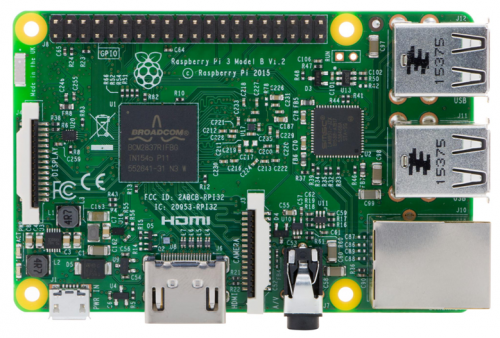
\includegraphics[width=100mm]{rpi.png}}
\end{center}

	\section{Workflow-ul normal pentru tipărire}
Un scenariu normal de printare prin CUPS presupune trimiterea pur si simplu a unui job de print catre CUPS, iar acesta se va ocupa de restul. Un aspect important este abstractizarea imprimantelor in spatele 'cozilor' CUPS si se urmareste ca acest aspect sa ramana neschimbat. CUPS asigneaza fiecarei imprimante una sau mai multe 'cozi' (queues), iar acestea apar ca imprimante pe retea pentru sistemele Unix (OSX, GNU/Linux, BSD, etc.).
Proiectul urmareste extragerea cat mai multor informatii din procesul normal de printare CUPS, dar si mentinerea modificarilor asupra CUPS la un nivel minim. O cerinta importanta este ca workflow-ul normal de printare sa ramana neschimbat, iar modificarile aduse pentru colectarea de date sa impacteze cat mai putin platforma.

\begin{center}
{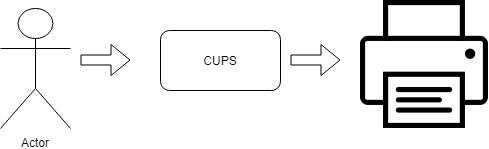
\includegraphics[width=110mm]{workflow.png}}
\end{center}

Modificarile aduse CUPS trebuie sa se respecte urmatoarele cerinte:
\begin{itemize}
\item sa nu adauge overhead sistemului
\item sa nu expuna informatie proprietara Océ
\item sa nu modifice functionarea modulelor CUPS
\item sa expuna intr-o maniera usor de interceptat informatiile relevante
\item sa respecte licenta Apache v2.0 aferenta CUPS
\end{itemize}

	\section{Colectarea și stocarea datelor}
Modificarile aduse CUPS urmaresc exclusiv colectarea datelor de imprimare si trimiterea lor catre agregator. Colectarea datelor se face intr-o maniera cat mai putin invaziva, conform cerintelor anterior mentionate. Se urmareste extragerea datelor spre a fi procesate, nu stocarea lor propriu zisa. Datele sunt transmise printr-un named pipe, prin urmare acestea nu parasesc niciodata siguranta nucleului sistemului de operare. Dupa ce datele sunt receptionate si procesate de catre agregator, acestea nu sunt salvate pe disc sau in alt mediu de stocare persistenta. Singurul loc in care datele persista este in Elasticsearch, dar este importanta mentiunea ca datele ajunse in Elasticsearch sunt deja procesate, iar in procesul de procesare pot fi eliminate orice informatii nedorite. 

Un alt criteriu important pe care proiectul a trebui sa il respecte este respectarea confidentialitatii datelor. In niciun punct sistemul nu colecteaza date cu caracter personal, nici macar numele utilizatorului, jobului sau masina de pe care a fost trimis un print job. 

\chapter{Design și implementare}

	\section{Arhitectură high-level}
		\begin{center}
			{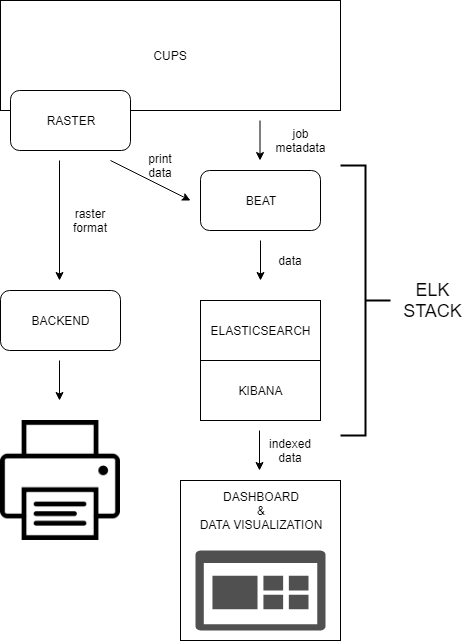
\includegraphics[width=110mm]{cups.png}}
		\end{center}
	\section{Componente software}
		\subsection{Sistemul de operare gazdă - BuruX}
Folosind CUPS ca backbone pentru sistem, s-a facut evidenta nevoie folosirii unui sistem de operare Unix-like care sa il gazduiasca. Pe considerente de familiaritate s-a ales folosirea unui sistem de operare bazat pe nucleul Linux. 
Nucleul Linux este un nucleu monolitic, adica lucreaza in intregime separat de restul sistemului si in mod administrator. Driverele se pot incarca in memoria de lucru la utilizare, de unde sunt sterse ulterior. Nucleul ofer facilitati precum:
\begin{itemize}
\item multitasking
\item suport pentru memorie virtuala
\item suport avansat pentru TCP/IP
\item sistem de sunet
\item pana la 1 miliard de procese simultane
\item management avansat si eficient al memoriei
\item suport pentru sistem multi-procesor
\end{itemize}

Distributia a fost compilata pentru ahritectura ARM, specifica procesorului Broadcom BCM2837 cu 4 nuclee ARM Cortex-A53, spre a fi instalata pe o placa Raspberry Pi 3. Procesorul si memoria de 1GB ale placii sunt mai mult decat suficiente pentru a rule sistemul de operare si componentele mentionate mai sus. Versiunea de kernel folosita este 4.14, cu niste patch-uri suplimentare care sa permita folosirea modulelor Bluetooth si Wi-Fi ale placii. In testele efectuate, sistemul de operare este perfect stabil si consuma foarte putine resurse comparativ cu o distributie de Linux full blown. Compilarea completa a sistemului de operare se face, pe o masina relativ veche, in sub 25 minute. Nucleul linux este principala componenta a sistemului de operare GNU/Linux. Pentru use-case-ul de fata, am ales sa nu instalez un desktop environment sau interfata grafica pe sistem, pe considerente de reducere a resurselor consumate. 
 Distributia de Linux folosita a fost compilata special pentru acest uz, drept urmare majoritatea functiilor au fost eliminate, ramanand doar cu cele strict esentiale pentru functionarea CUPS:
\begin{itemize}
\item facilitati elementare de networking - Avahi
\item o selectie minimala de unelte si compilatoare - clang, golang
\item sistemul de printing CUPS cu dependentele aferente
\item functionalitate de remote access - SSH
\end{itemize}

Pentru compilare si aplicare de patch-uri a fost folosit Buildroot - o unealta care automatizeaza procesul de building al unui mediu Linux complet si bootabil, folosind cross-compilation pentru a putea servi multiple platforme. Buildroot isi poate build-ui propriul toolchain, crea un root file system, compila o imagine de Linux kernel si genera un boot loader pentru sistemul dorit. Acesta functioneaza pe baza unor fisiere de configuratii, numite defconfigs, care contin informatii relevante pentru procesul de build (versiune de kernel, arhitectura, target file system, etc.). Sunt suportate mai multe biblioteci de C, printre care GNU C Library, uClibc si musl. Intern, Buildroot foloseste Kconfig pentru sistemul de configuratie, acesta oferind facilitati precum o interfata cu meniu, ocuparea de dependente, optiunea de 'Help' contextual. Intregul proces de build se construieste in jurul pachetelor descarcate automate in functie de defconfig. Aceste pachete pot include aplicatii, utilitati, biblioteci, etc. Rezultatul final este un root file system care poate fi copiat pe un mediu bootabil si folosit as-is. Buildroot face tot procesul de compilare, build si deployment usor de inteles si accesibil oricui. 

Pe parcurs, a aparut problematica alegerii unui sistem de init. Buildroot pune la dispozitie implicit BusyBox - o implementare a unui program rudimentar de init, suficient pentru majoritatea aplicatiilor.
		\subsection[CUPS]{CUPS\\ {\normalsize Common UNIX Printing System}}
Aparut in 1999, CUPS este un sistem modular de printing open-source pentru sistemele de operare Unix-like. Acesta permite unui calculator sa se comporte ca un print server, devenind un host care accepta job-uri de la clienti, le proceseaza si le trimite catre imprimante.
CUPS este format dintr-un spooler, un scheduler, un sistem de filtre care transforma datele dintr-un format in altul, si un sistem de backend-uri care realizeaza comunicarea cu imprimantele.

Workflow-ul standard CUPS este urmatorul: un job ajunge in scheduler, acesta il trimite catre unul sau mai multe filtre spre a fi convertit in alt format, apoi datele ajung intr-un backend de unde sunt trimise spre printer. Sistemul foloseste extensiv PostScript si rasterizarea datelor ca formate intelese de imprimante.
			\subsubsection{Scheduler-ul CUPS}
Scheduler-ul CUPS implementeaza Internet Printing Protocol si ofera o interfata web-based pentru managementul imprimantelor, job-urilor, configuratii server si documentatie. Pentru accesarea functionalitatilor de management si configuratie, un utilizator trebuie sa se autentifice. 
O alta parte foarte importanta a scheduler-ului este modulul de logging. Acesta inregistreaza evenimente legate de acces, erori sau page log.
Alte module importante ale schedeuler-ului sunt: modulul MIME (multipurpose internet mail extensions), modulul PPD (PostScript printer description), modulul care se ocupa cu management-ul dispozitivelor disponibile in sistem.


			\subsubsection{Sistemul de filtre CUPS}
Sistemul de filtre al CUPS poate procesa o varietate de formate. Acesta converteste datele unui print-job intr-un limbaj/format final printr-un sistem de filtre, folosind MIME types pentru identificarea formatelor.
Procesul de filtrare incepe prin determinarea tipului de date de intrare, folosind MIME databases. Printre filtrele default ale CUPS se numara: raster to PCL, raster to ESC/P, raster to Dymo, raster to ZPL.
Initial, am incercat modificare scheduler-ului, mai exact a modulului de logging, dar informatiile pe care le puteam obtine din acesta erau insuficiente pentru cerintele proiectului, in modulul de logging fiind expuse numai date despre utlizatori, job-uri sau status. Considerand nevoia de a obtine date despre pixeli, culoare, media, pagina, etc. s-a facut necesara accesarea informatiilor disponibile in sistem de filtre al CUPS, mai exact in unitatea de raster. Dupa ce am identificat informatiile de care am nevoie, le-am trimis catre exterior printr-un HTTP POST, apoi printr-un named pipe. Folosind un apel de sistem catre comanda cURL pentru a trimite cererea HTTP catre Beat, s-ar fi creat un numar de procese greu de controlat si care ar fi generat overhead pe care il puteam evita. O a doua alternativa ar fi fost folosirea unei biblioteci, de exemplu libcurl, pentru a inlocui apelurile de sistem, dar aceasta alternativa ar fi introdus o dependenta suplimentara in CUPS, ceea ce ar fi facut codul mai putin portabil si ar fi incalcat una din cerintele initiale ale proiectului. In final, am folosit un named pipe pentru transmiterea datelor, acesta fiind usor de accesat si generand overhead minim, iar in plus, datele nu sunt expuse in retea, aceasta interfata rezidand in kernelul sistemului de operare.


			\subsubsection{Backend-urile CUPS}
Backend-urile CUPS sunt folosite pentru a trimite datele catre imprimante. CUPS pune la dispozitie multe backend-uri: paralel, serial, USB, cups-pdf, PDF virtual printing, JetDirect, LPD, SMB, etc.
		
		
		\subsection[Elastic Stack]{Elastic Stack\\ {\normalsize Beater - Elasticsearch - Kibana}}
Elastic Stack este o stiva de aplicatii care permite extragerea, procesarea si vizualizarea datelor. In majoritatea cazurilor, acesta este gasit sub numele de ELK Stack (Elasticsearch - Logstash - Kibana). Pentru aceasta teza nu a fost folosit Logstash, fiind inlocuit cu un Elastic Beater ca unealta de colectare a datelor. Un Beat implementeaza interfata Beater si aduna date spre a le trimite catre Kibana sau, in cazul de fata, Elasticsearch.


			\subsubsection{Beat}
Beat-urile au fost adaugate recent la stack-ul ELK. Un Beat are responsabilitatea sa colecteze date si sa le trimita spre procesare sau vizualizare. Acesta trebuie sa implementeze in Golang o interfata numita Beater interface, care contine metode de Start, Run si Stop. Aceasta lucrare foloseste un Beat pentru a primi date de la raster-ul, raster care face parte din sistemul de filtre mentionat anterior. Beat-ul primeste raster data, face operatii de procesare si sanitization minimale, apoi trimite datele catre Elasticsearch. In implementarile conventionale de Beat, datele sunt transimse la intervale periodice de timp catre Elasticsearch sau Kibana. Implementarea Beat-ului din aceasta lucrare trimite date catre Elasticsearch atunci cand primeste informatii noi de la raster. cBeat (Beater-ul implementat pentru aceasta lucrare) urmatoarele componente principale:
\begin{outline}
\1 {\large Metodele interfetei Beater}
	\2
	\textbf{metoda Run}
		\3 contine bucla principala a aplicatiei
		\3 in interiorul buclei se transmit evenimente catre restul ELK stack
		\3 un eveniment este trimis encodat ca JSON catre Elasticsearch
		\3 mai jos este exemplificata metoda Run din exemplul oferit de Elastic
		\3 se observa cum evenimentel sunt trimise la intervale periodice de timp
\begin{lstlisting}[caption={exemplu metoda Run - golang},captionpos=b]
func (bt *Countbeat) Run(b *beat.Beat) error {
        logp.Info("countbeat is running! Hit CTRL-C to stop it.")

        bt.client = b.Publisher.Connect()
        ticker := time.NewTicker(bt.config.Period)
        counter := 1
        for {
                select {
                case <-bt.done:
                        return nil
                case <-ticker.C:
                }

                event := common.MapStr{ 
                        "@timestamp": common.Time(time.Now()), 
                        "type":       b.Name,
                        "counter":    counter,
                }
                bt.client.PublishEvent(event) 
                logp.Info("Event sent")
                counter++
        }
}
\end{lstlisting}

	\2
	\textbf{metoda Stop}
		\3 este chemata atunci cand Beat-ul e semnalat sa se opreasca
		\3 mai jos este exemplificata metoda Stop
\begin{lstlisting}[caption={exemplu metoda Stop - golang},captionpos=b]
func (bt *Countbeat) Stop() {
        bt.client.Close()
        close(bt.done)
}
\end{lstlisting}
\1  {\large Receptionarea datelor din CUPS}
	\2 citirea din named pipe a evenimentelor se face prin deschiderea FIFO-ului ca orice alt fisier de pe disk, folosind modulul os al Golang
\begin{lstlisting}[caption={deschidere named pipe - golang},captionpos=b]
pipePath = "/tmp/cupsbeat"
 if p, err = os.Open(pipePath); os.IsNotExist(err) {
     log.Fatalf("Named pipe '\%s' does not exist", pipePath)
} else if os.IsPermission(err) {
    log.Fatalf("Insufficient permissions to read named pipe '\%s': \%s", pipePath, err)
} else if err != nil {
    log.Fatalf("Error while opening named pipe '\%s': \%s", pipePath, err)
}
defer p.Close()
\end{lstlisting}

	\2 FIFO-ului i s-a adaugat un mecanism de watch care ne notifica atunci cand s-a efectuat orice scriere in pipe
\begin{lstlisting}[caption={watch pentru named pipe - golang},captionpos=b]
c := make(chan notify.EventInfo, MAX_CONCURRENT_WRITERS)
notify.Watch(pipePath, c, notify.Write|notify.Remove)
\end{lstlisting}

	\2 functia care supravegheaza pipe-ul a fost lansata intr-o go rutina in metoda Run
\begin{lstlisting}[caption={apel readPipe in go routina separata - golang},captionpos=b]
go func(){
	readPipe()
}()
\end{lstlisting}
	\2 ca mecanism IPC s-a folosit un go channel intre green thread-ul care citeste din pipe si cel al metodei principale
\begin{lstlisting}[caption={instantiere canal - golang},captionpos=b]
var messageQueue = make(chan Message_s_t)
\end{lstlisting}

\1 {\large Generarea structurilor necesare prelucrarii datelor}
	\2 pe baza enum-urilor definite in CUPS se urmareste generarea unor structuri de date echivalente in limbajul Go
\begin{lstlisting}[caption={exemplu enum CUPS - C},captionpos=b]
typedef enum cups_adv_e			/**** AdvanceMedia attribute values ****/
{
  CUPS_ADVANCE_NONE = 0,		/* Never advance the roll */
  CUPS_ADVANCE_FILE = 1,		/* Advance the roll after this file */
  CUPS_ADVANCE_JOB = 2,			/* Advance the roll after this job */
  CUPS_ADVANCE_SET = 3,			/* Advance the roll after this set */
  CUPS_ADVANCE_PAGE = 4			/* Advance the roll after this page */
} cups_adv_t;

\end{lstlisting}
	\2 pentru transmiterea eficienta a datelor, se pastreaza encodarea diferitor optiuni de tiparire in numere intregi
	\2 generarea de cod Go din fisierele header care contin structurile CUPS presupune parcurgerea lor
	\2 rezultatul final trebuie sa fie un fisier .go compilabil care contine structurile echivalente
	\2 s-a folosit un algoritm similar cu un automate care parcurge fisierul
	\2 automatul salveaza fiecare intrare intr-un dictionar de dictionare de siruri de caractere
\begin{lstlisting}[caption={instantiere dictionar - golang},captionpos=b]
var maps = make(map[string]map[string]string)
\end{lstlisting}
	\2 fiecare intrare corespunde unui enum, cu dictionarul corespunzator
	\2 intrarile din dictionarul corespunzator reprezinta prechile de intregi - sir de caractere
	\2 intregul modul de generare de cod a fost scris in limbajul Go
\begin{lstlisting}[caption={structuri de date pentru generator/procesor date - golang},captionpos=b]
type HWResolution_t struct {
	Hr1 int
	Hr2 int
}

type ImaginBoundingBox_t struct {
	Ibb1 int
	Ibb2 int
	Ibb3 int
	Ibb4 int
}

type PageSize_t struct {
	Ps1 int
	Ps2 int
}

type Message_t struct{
	CutMedia int
	Duplex int
	HWResolution HWResolution_t
	ImagingBoundingBox ImaginBoundingBox_t
	InsertSheet int
	Orientation int
	NumCopies int
	PageSize PageSize_t
	Tumble int
	CupsWidth int
	CupsHeight int
	CupsBitsPerColor int
	CupsBitsPerPixel int
	CupsColorOrder int
	CupsColorSpace int
	CupsNumColors int
}

type Message_s_t struct{
	CutMedia string
	Duplex int
	HWResolution HWResolution_t
	ImagingBoundingBox ImaginBoundingBox_t
	InsertSheet int
	Orientation string
	NumCopies int
	PageSize PageSize_t
	Tumble int
	CupsWidth int
	CupsHeight int
	CupsBitsPerColor int
	CupsBitsPerPixel int
	CupsColorOrder string
	CupsColorSpace string
	CupsNumColors int
}
\end{lstlisting}

\1 {\large Prelucrarea datelor}
	\2 la compilare, se populeaza structurile mentionate la punctul anterior pe baza header-ului CUPS
	\2 atunci cand se receptioneaza un eveniment, avesta ajunge in Beat sub forma de string
	\2 evenimentul este procesat pe baza dictionarelor, intregii fiind inlocuiti cu stringuri
	\2 dupa prelucrare, evenimentul este serializat ca JSON si este trimis catre Elasticsearch

\begin{lstlisting}[caption={functia pentru procesarea mesajelor - golang},captionpos=b]
func processMsg(msg string) Message_s_t{
	var maps = cups_itf.Maps
	fmt.Println(maps["Duplex"]["0"])
	logp.Info("PROCESSING STRING:")
	logp.Info(msg)
	var message Message_t
	var message_s Message_s_t
	if isJSON(msg){
		logp.Info("VALID JSON")
		json.Unmarshal([]byte(msg), &message)
		message_s.CutMedia = maps["CutMedia"][strconv.Itoa(message.CutMedia)]
		message_s.Duplex = message_s.Duplex
		message_s.HWResolution = message.HWResolution
		message_s.ImagingBoundingBox = message.ImagingBoundingBox
		message_s.InsertSheet = message.InsertSheet
		message_s.Orientation = maps["Orientation"][strconv.Itoa(message.Orientation)]
		message_s.NumCopies = message.NumCopies
		message_s.PageSize = message.PageSize
		message_s.Tumble = message.Tumble
		message_s.CupsWidth = message.CupsWidth
		message_s.CupsHeight = message.CupsHeight
		message_s.CupsBitsPerColor = message.CupsBitsPerColor
		message_s.CupsBitsPerPixel = message.CupsBitsPerPixel
		message_s.CupsColorOrder = maps["cupsColorOrder"][strconv.Itoa(message.CupsColorOrder)]
		message_s.CupsColorSpace = maps["cupsColorSpace"][strconv.Itoa(message.CupsColorSpace)]
		message_s.CupsNumColors = message.CupsNumColors
		logp.Info("CREATED NEW STRUCT")
	}
	return message_s
}
\end{lstlisting}
\end{outline}


			\subsubsection{Elasticsearch}
Elasticsearch este un motor de cautare bazat pe Apache Lucene. Ofer clienti disponibili in majoritatea tehnologiilor si este cel mai popular motor de cautare enterprise. Beneficiile Elasticsearch includ: cautare foarte scalabila, aproape real-time, suportul mai multor clienti, platforma distribuita. Este considerat de multi backbone-ul stack-ului ELK. Informatiile extrase de Beat ajung in Elasticsearch, iar acesta cauta tipare si indexeaza datele spre a le trimite catre Kibana.


			\subsubsection{Kibana}
Kibana este un plugin open source pentru vizualizare de data, care pune la dispozitie capabilitati de vizualizare ale elementelor indexate intr-un cluster Elasticsearch. Un utilizator poate  construi diferite tipuri de grafice bazate pe datele indexate de Elasticsearch, iar pe baza acestor grafice se pot construi dashboard-uri configurabile. Kibana preia datele indexat de la Elastisearch si le foloseste la generarea de grafice si vizualizari relevante pentru utilizator.

Atat Elasticsearch, cat si Kibana sunt hostate pe o masina (Debian) in cloud pe platforma Scaleway. Masina are o configuratie minimala, stack-ul fiind unul robust si eficient nu are nevoie de multe resurse. Administrarea masinii se face strict prin SSH, iar interfata web Kibana este expusa spre exterior. Prin intermediul aplicatiei web se face si configurarea graficelor si dashboard-ului Kibana. Pe masina host este instalat nginx care redirecteaza orice acces HTTP catre portul Kibana (9300).
	\section{Comunicarea între module}

\chapter{Rezultate}

\chapter{Concluzii}

\chapter{Glosar de termeni}
\begin{itemize}
\item \acrshort{cups} - \acrlong{cups}
\item PDF - 
\item GNU - 
\item Linux -  
\item OSX - 
\item BSD - 
\item kernel - 
\item Avahi - 
\item golang - 
\item clang - 
\item Elastic stack - ELK stack - 
\item Kibana - 
\item Elasticsearch - 
\item nginx -
\end{itemize}

\chapter{Referințe}

\clearpage

\printglossaries
\end{document}
